\documentclass[letterpaper]{article}
\usepackage[utf8]{inputenc}
\usepackage[spanish]{babel}
\usepackage[letterpaper,includeheadfoot, top=.5cm, bottom=3.0cm, right=2.0cm, left=2.0cm]{geometry}
\renewcommand{\familydefault}{\sfdefault}
\usepackage{amsmath}
\usepackage{graphicx}
\usepackage{subcaption}
\usepackage{gensymb}
\usepackage{color}
\usepackage{hyperref}
\usepackage{amssymb}
\usepackage{url}
%\usepackage{pdfpages}
\usepackage{fancyhdr}
\usepackage{enumerate}
\usepackage{float}
\usepackage{tikz}
\usepackage{siunitx}
\usepackage{framed}
\tikzset{
every picture/.append style={
  execute at begin picture={\deactivatequoting},
  execute at end picture={\activatequoting}
  }
}
%-------------------- CABECERA ---------------------
\pagestyle{fancy}
\fancyhf{}
\author{Martin Bataille}
\date{}
\title{\bf MCU Strikes Again}
%Encabezado
\fancyhead[R]{
\includegraphics[scale=0.35]{jct.jpg}}
\fancyfoot[C]{\thepage}


\newcommand{\tpb}[1]{node[midway, below, sloped] {#1}}
\newcommand{\tpa}[1]{node[midway, above, sloped] {#1}}
\newcommand{\tvec}[3]{[->, thick] #1 -- #2 \tpb{#3}}
\newcommand{\tveca}[3]{[->, thick] #1 -- #2 \tpa{#3}}
\newcommand{\tvecnotsloped}[3]{[->, thick] #1 -- #2 {node[midway, above] {#3}}}

\newcounter{propiedades}
\newcounter{definiciones}

\newcommand{\propi}{\stepcounter{propiedades} \textbf{Propiedad \thepropiedades}: }
\newcommand{\defii}{\stepcounter{definiciones} \textbf{Definición \thedefiniciones}: }

\newenvironment{prop}
{ \begin{framed} \propi}
{ \end{framed} }
\newenvironment{defi}{\begin{framed} \defii}{\end{framed}}

\renewcommand{\sectionmark}[1]{\markright{\thesection.\ #1}}
\renewcommand{\headrulewidth}{0.5pt}
\renewcommand{\footrulewidth}{0pt}
\setlength{\headheight}{92pt}

% --------------- ---------PORTADA -----------------------
\begin{document}
\maketitle
\thispagestyle{fancy}
\begin{center}
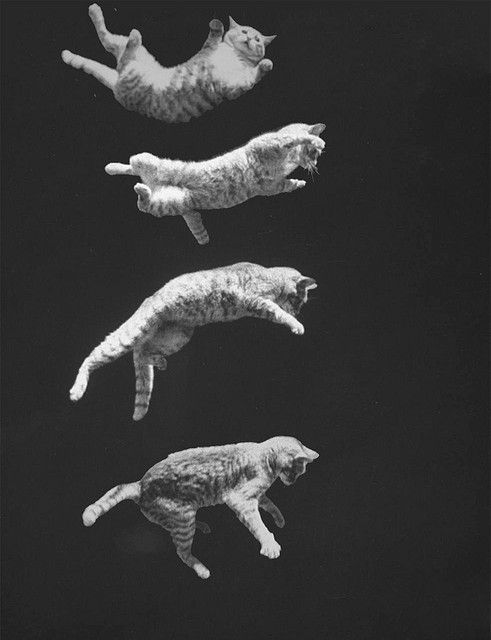
\includegraphics[scale=0.6]{portada.jpg}
\end{center}
\pagebreak

Los egipcios consideraban a los gatos como animales sagrados e incluso les asociaban propiedades mágicas. Cualquier dueño de un gato conoce la ternura de los gatos y la magia de su ronroneos, que pueden levantarte el ánimo incluso en los peores días. Pero los físicos se interesaron mucho en los gatos por otra razón. Por una pregunta que por siglos no conoció respuesta. ¿Cómo es que los gatos siempre caen parados? ¿Cómo es que partiendo del reposo, pueden girar espontáneamente? ¿Nosotros podemos hacer lo mismo? Todo esto y mucho más lo veremos a lo largo de la guía.  


\section*{Actividad paranormal: Fuerza centrífuga}

Probablemente una de las fuerzas más famosas es la que nos bota de las micros cuando giran muy rápido, la que nos permite secar la ropa en la secadora o la que nos empuja hacia afuera en una montaña rusa, así es: la fuerza centrífuga. Paradójicamente, ¡esta fuerza no existe! En física se le llama a este tipo de fuerzas, \emph{fuerzas virtuales} ya que no existen pero aún así se sienten como fuerzas. ¿Cómo se explica esto?


Para comprender el tema tenemos que saber lo que es un sistema inercial. Cuando vimos las leyes de Newton, la verdad es que esas leyes vienen con una letra chica: solo se aplican en un sistema inercial. ¿Qué es un sistema inercial? Pues un sistema en el que se aplican las leyes de Newton. De aquí surge una muy buena pregunta, ¿existe un sistema en donde no se cumplan las leyes de Newton? 

Podemos pensar en el metro, si dejas una maleta con ruedas en reposo en la mitad del metro, las únicas fuerzas que se aplican sobre la maleta son las fuerzas peso, normal, roce estático con el suelo (despreciable porque tiene ruedas) y roce con el aire (también despreciable). Sin embargo, sabemos que la maleta no se mueve verticalmente, por lo tanto, necesariamente la fuerza de peso es igual a la normal, mientras que en el eje horizontal no existe ninguna fuerza, o sea que, por la primera ley de newton, la maleta va a seguir en reposo. En la realidad, cuando el metro comienza a acelerar, la maleta se va al otro extremo del metro ya que se mantiene en reposo respecto a la estación de metro, no al metro en sí. El metro es entonces un sistema no inercial, ya que les las leyes de Newton no se cumplen, mientras que la estación de metro es un sistema inercial.

De manera general, un sistema es no inercial si acelera o rota con respecto a un sistema inercial. En el caso del metro, podemos pensar en la estación de metro como un sistema inercial ya que, efectivamente, las leyes de Newton se cumplen en la estación de metro, y, puesto que el metro está acelerando con respecto a la estación, el metro deja de ser un sistema inercial. Para poder aplicar las leyes de Newton en un sistema no inercial, hay que agregar fuerzas \emph{ficticias} o \emph{virtuales}, como la fuerza centrífuga. De esta manera, para estudiar el movimiento de la maleta, hay que introducir una fuerza ficticia que sería la responsable de que la maleta se escape al otro extremo del metro.                   

                                                                                                                                  
\section*{Ejercicios}

\begin{enumerate}

\item Una piedra de masa $m$, gira en MCU con una frecuencia $f$ y un radio $R$. Con esta información podemos determinar la magnitud de:

\begin{enumerate}[I]
\item La aceleración centrípeta
\item La fuerza centrípeta sobre la piedra
\item El momentum angular
\end{enumerate}

\begin{enumerate}[label=\Alph*)]
\item Sólo I
\item Sólo I y II
\item Sólo I y III
\item Sólo II y III
\item Sólo II y III
\item I, II y III
\end{enumerate}

\end{enumerate}

\section*{Problemas}

\begin{enumerate}

\item Pendiente

\end{enumerate}

\end{document}